\chapter{Case Study in CSDL} \label{Chapter:EvaluationInCSDL}


This chapter describes a case study that will be conducted in Collaborative Software Development Lab at University of Hawaii, where a large scale software project (100 KSLOC) is being developed and maintained. The project has experienced a significant rate of integration build failure (88 failures out of 300 builds in 2004). The case study has dual objectives: 

\begin{itemize}
	\item To use software project telemetry to understand and improve CSDL build process.
	\item To evaluate software project telemetry at the same time in CSDL (an environment typical of traditional software development with close collaboration and centralized decision-making). 
\end{itemize}



This chapter begins with a description of CSDL environment and its build problem in Section \ref{EvaluationInCSDL:Setting}.
Section \ref{EvaluationInCSDL:Role} introduces case study participants and the researcher's role.
Section \ref{EvaluationInCSDL:Design} outlines the design and strategies of this case study and offers rationale for the decisions.
Section \ref{EvaluationInCSDL:DataAnalysis} describes data collection and analysis procedures.
Section \ref{EvaluationInCSDL:Threats} discuses the limitations and threats. 
The expected results are described in Section \ref{EvaluationInCSDL:Results}.
%and the time frame of this case study is given in Section \ref{EvaluationInCSDL:TimeFrame}.
 
 

%%%%%%%%%%%%%%%%%%%%%%%%%%%%%%%%%%%%%%%%%%%%%%%%%%%%%%%%%
%                                                       %
%                   S E C T I O N                       %
%                                                       %
%%%%%%%%%%%%%%%%%%%%%%%%%%%%%%%%%%%%%%%%%%%%%%%%%%%%%%%%%

\section{CSDL Setting}  \label{EvaluationInCSDL:Setting}

The Collaborative Software Development Laboratory (CSDL) is a software engineering research lab at University of Hawaii. Its mission is to provide a physical, organizational, technological, and intellectual environment conductive to collaborative development of software engineering skills. Hackystat is a software system developed and maintained by CSDL. Its aim is to provide a common framework for automated metrics collection and software engineering experimentation. %It has been under active development since 2001. 




%%%%%%%%%%%%%%%%%%%%%%%%%%%%%%%%%%%%%%%%%%%%%%%%%%%%%%%%%
%           S U B   S E C T I O N                       %
%%%%%%%%%%%%%%%%%%%%%%%%%%%%%%%%%%%%%%%%%%%%%%%%%%%%%%%%%

\subsection{Build Process}

Hackystat consists of over 100 thousand lines of code at the time of this writing. The code is organized into over 30 different modules, with 5 -- 10 active developers. The sources are stored in a central version control repository, which supports concurrent development by allowing developers to checkout the latest version of the sources and commit their changes. Developers rarely compile, build, and test the system against the entire code base. Instead, they often work with a subset of the modules relevant to their assignments. 

In order to handle full system build and test, I designed and implemented an automated integration build tool, which checks out the latest version of the entire code base, compiles, builds, and tests the system. The build tool is designed so that it starts the integration build automatically at night if it detects any change in the code repository in the previous day. If there is any build error, an email is sent to the development team. Figure \ref{fig:BuildProcess} is a graphical illustration of the build process.

\begin{figure}[p]
  \centering
  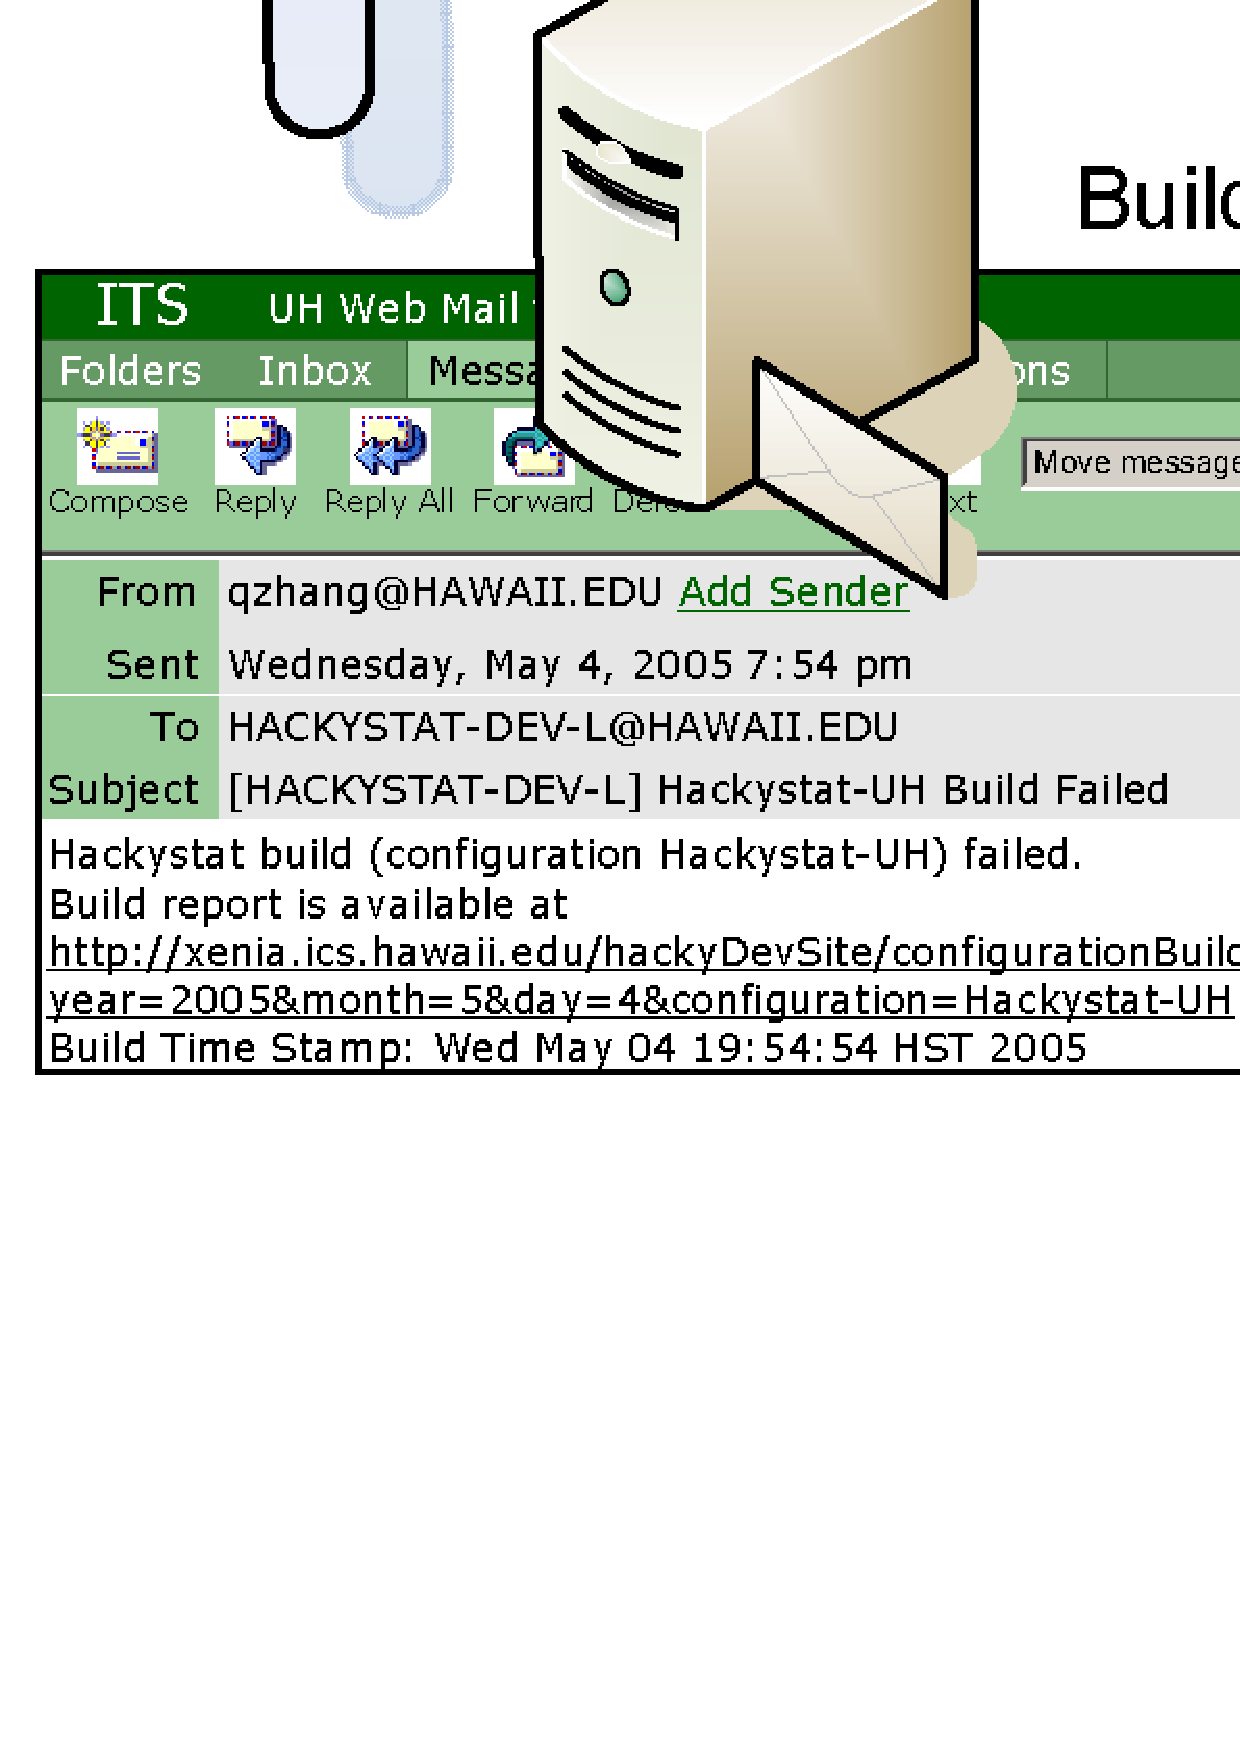
\includegraphics[width=1.00\textwidth]{figures/BuildProcess}
  \caption{Hackystat Build Process}
  \label{fig:BuildProcess}
\end{figure}

\newpage

%%%%%%%%%%%%%%%%%%%%%%%%%%%%%%%%%%%%%%%%%%%%%%%%%%%%%%%%%
%           S U B   S E C T I O N                       %
%%%%%%%%%%%%%%%%%%%%%%%%%%%%%%%%%%%%%%%%%%%%%%%%%%%%%%%%%

\subsection{Build Problem}

The automated build tool was deployed in CSDL in the summer of 2003. At the end of 2004, I conducted a study on the build results and found that integration build failure rate was significant. There were 300 days in which Hackystat code repository was changed for the entire year of 2004. As a result, there were 300 integration build attempts by the automated build tool. Out of those 300 build attempts, the build failed 88 times with a total of 95 errors. 

Figure \ref{fig:WeeklyBuildFailuresAndAttempts2004} shows the build failure information on a weekly basis. The top line indicates the number of build attempts in each week. Since the automated build tool initiates an integration build only when it detects source code change in the previous day, the maximum number of build attempts in a week is seven. The bottom lines represents the number of build failures in each week. A few weeks saw 100\% build failure (e.g. week 16 -- 17), while a few other weeks saw 100\% build success (e.g. week 19 -- 22). In most weeks, the build failure rate fluctuated between 20\% to 50\%. The overall average failure rate was 29.33\%. 

The loss of productivity due to the integration build failures was substantial, since each build failure generally required one or more developers to stop concurrent development, diagnose the problem, and determine who was responsible for fixing the error. Often times, other developers had to wait until the corrections were made before they could check out or commit additional code.

%\textcolor{red}{[TODO: Figure \ref{fig:WeeklyBuildFailureCount2004} and \ref{fig:WeeklyBuildFailureRatio2004} will be redrawn using curring telemetry chart format. Build attempt count should be added to the first figure.]}

\begin{figure}[tbp]
  \centering
  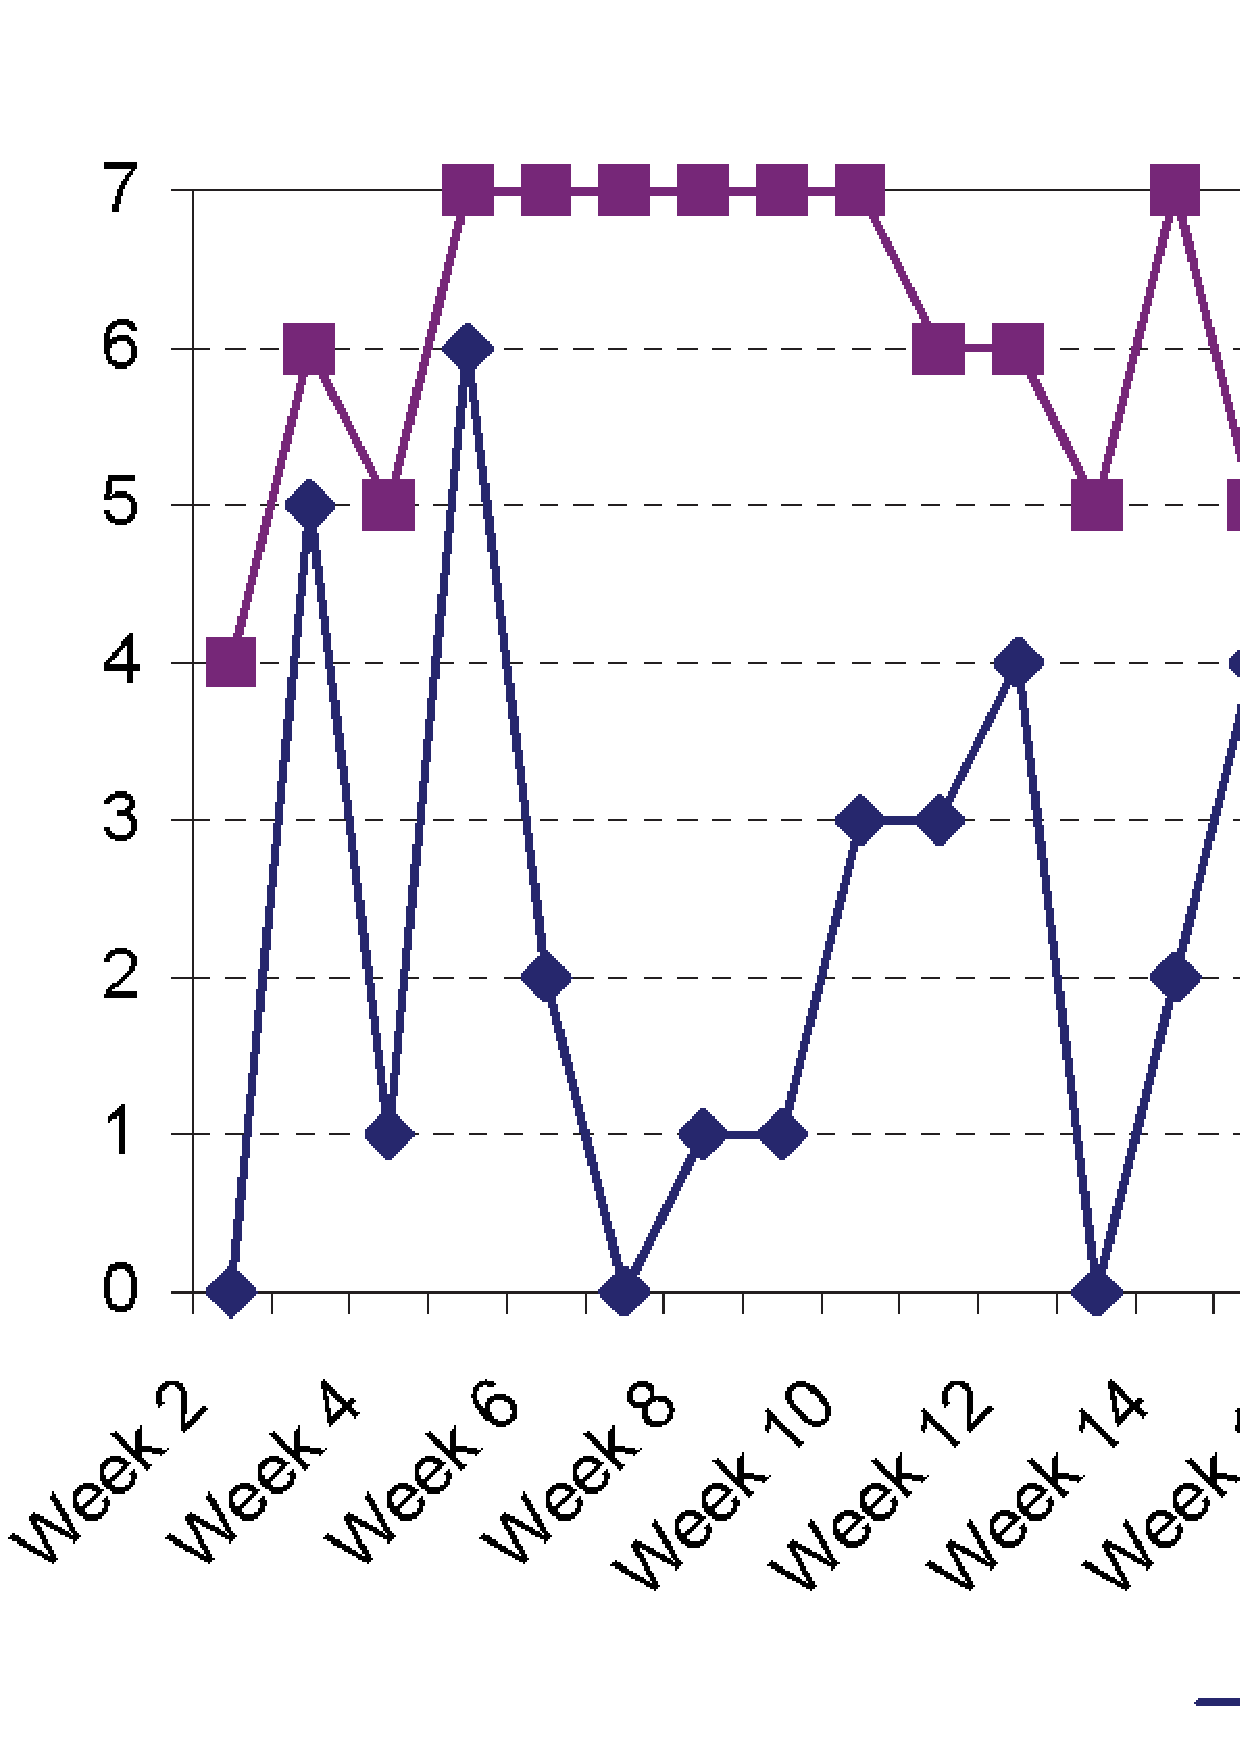
\includegraphics[width=1.00\textwidth]{figures/WeeklyBuildFailuresAndAttempts2004}
  \caption{Weekly Hackystat Build Failures and Attempts for the Year 2004}
  \label{fig:WeeklyBuildFailuresAndAttempts2004}
\end{figure}

%\begin{figure}[p]
%  \centering
%  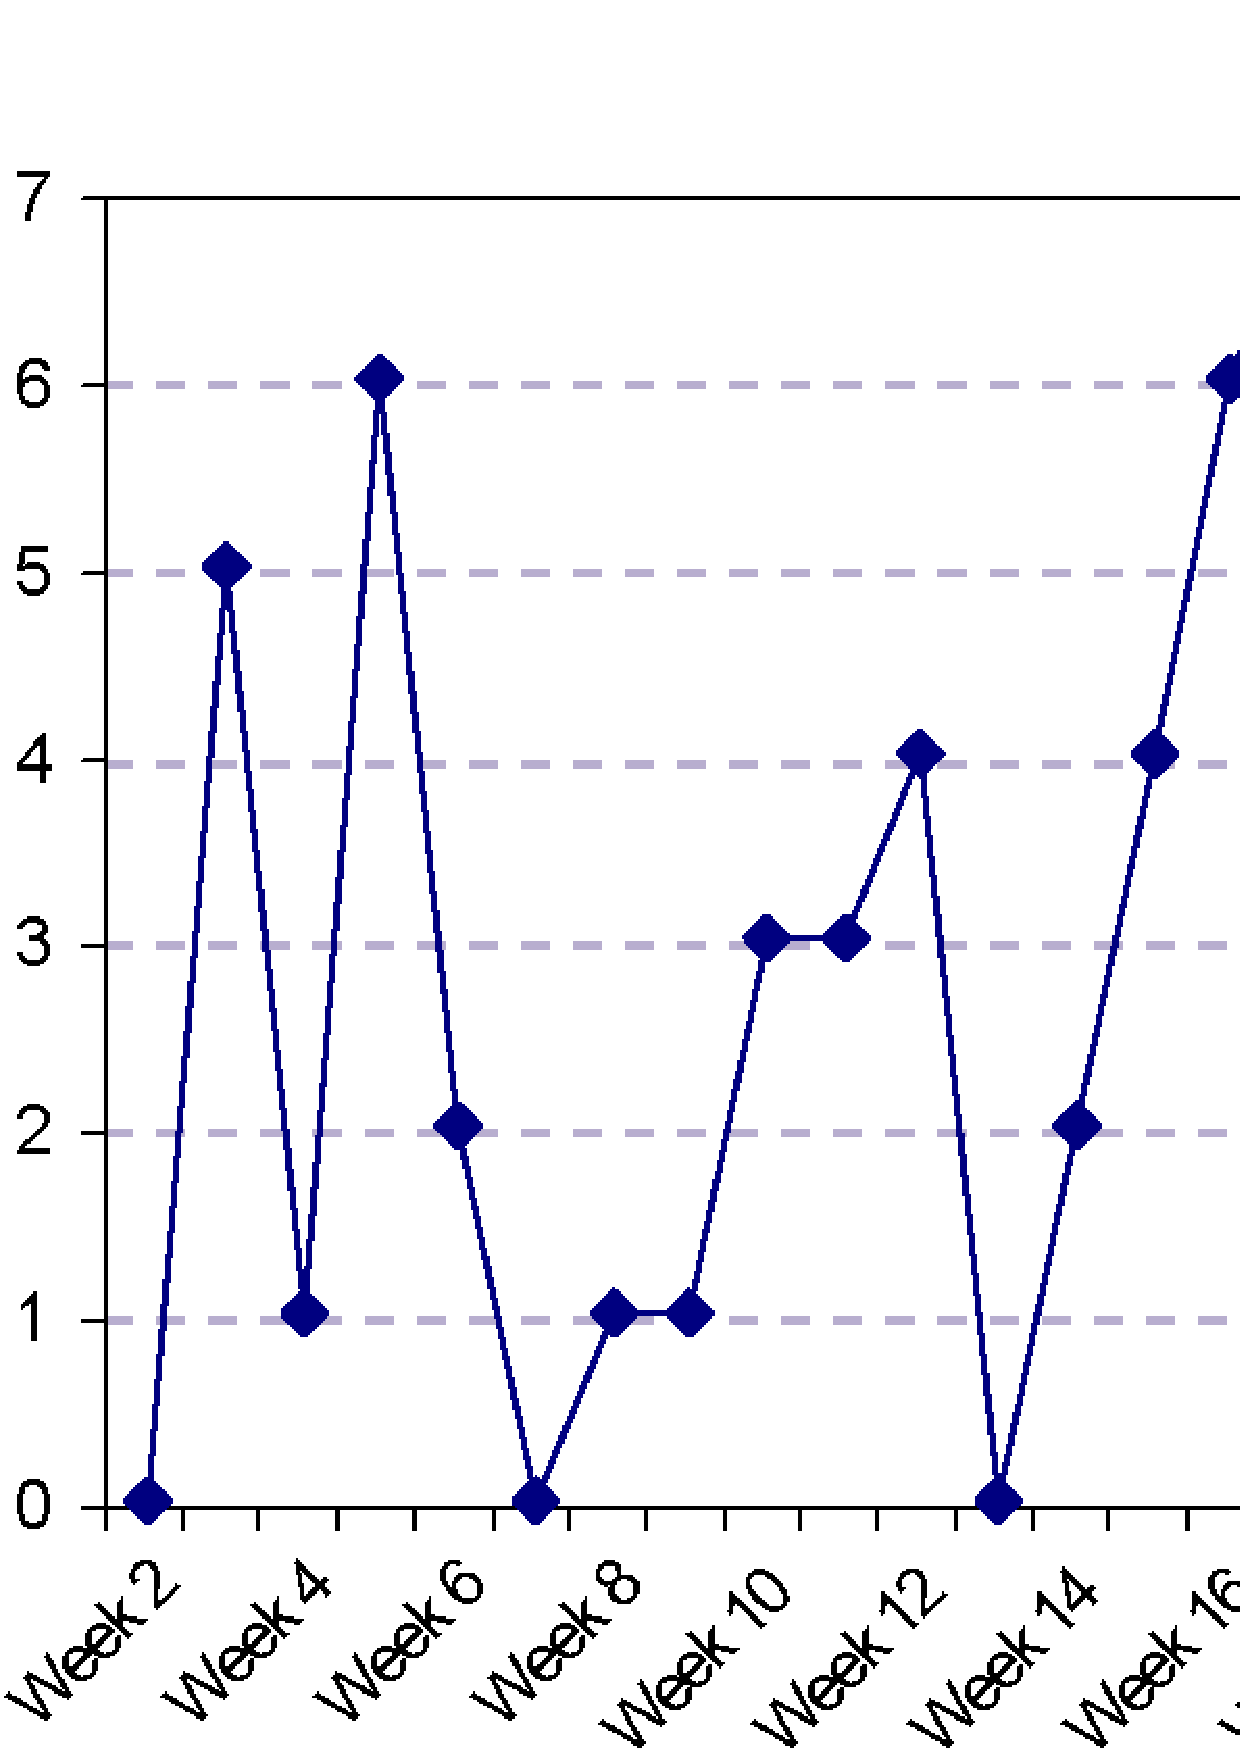
\includegraphics[width=1.00\textwidth]{figures/WeeklyBuildFailureCount2004}
%  \caption{Weekly Hackystat Build Failure Count for the Year 2004}
%  \label{fig:WeeklyBuildFailureCount2004}
%\end{figure}
%
%\begin{figure}[p]
%  \centering
%  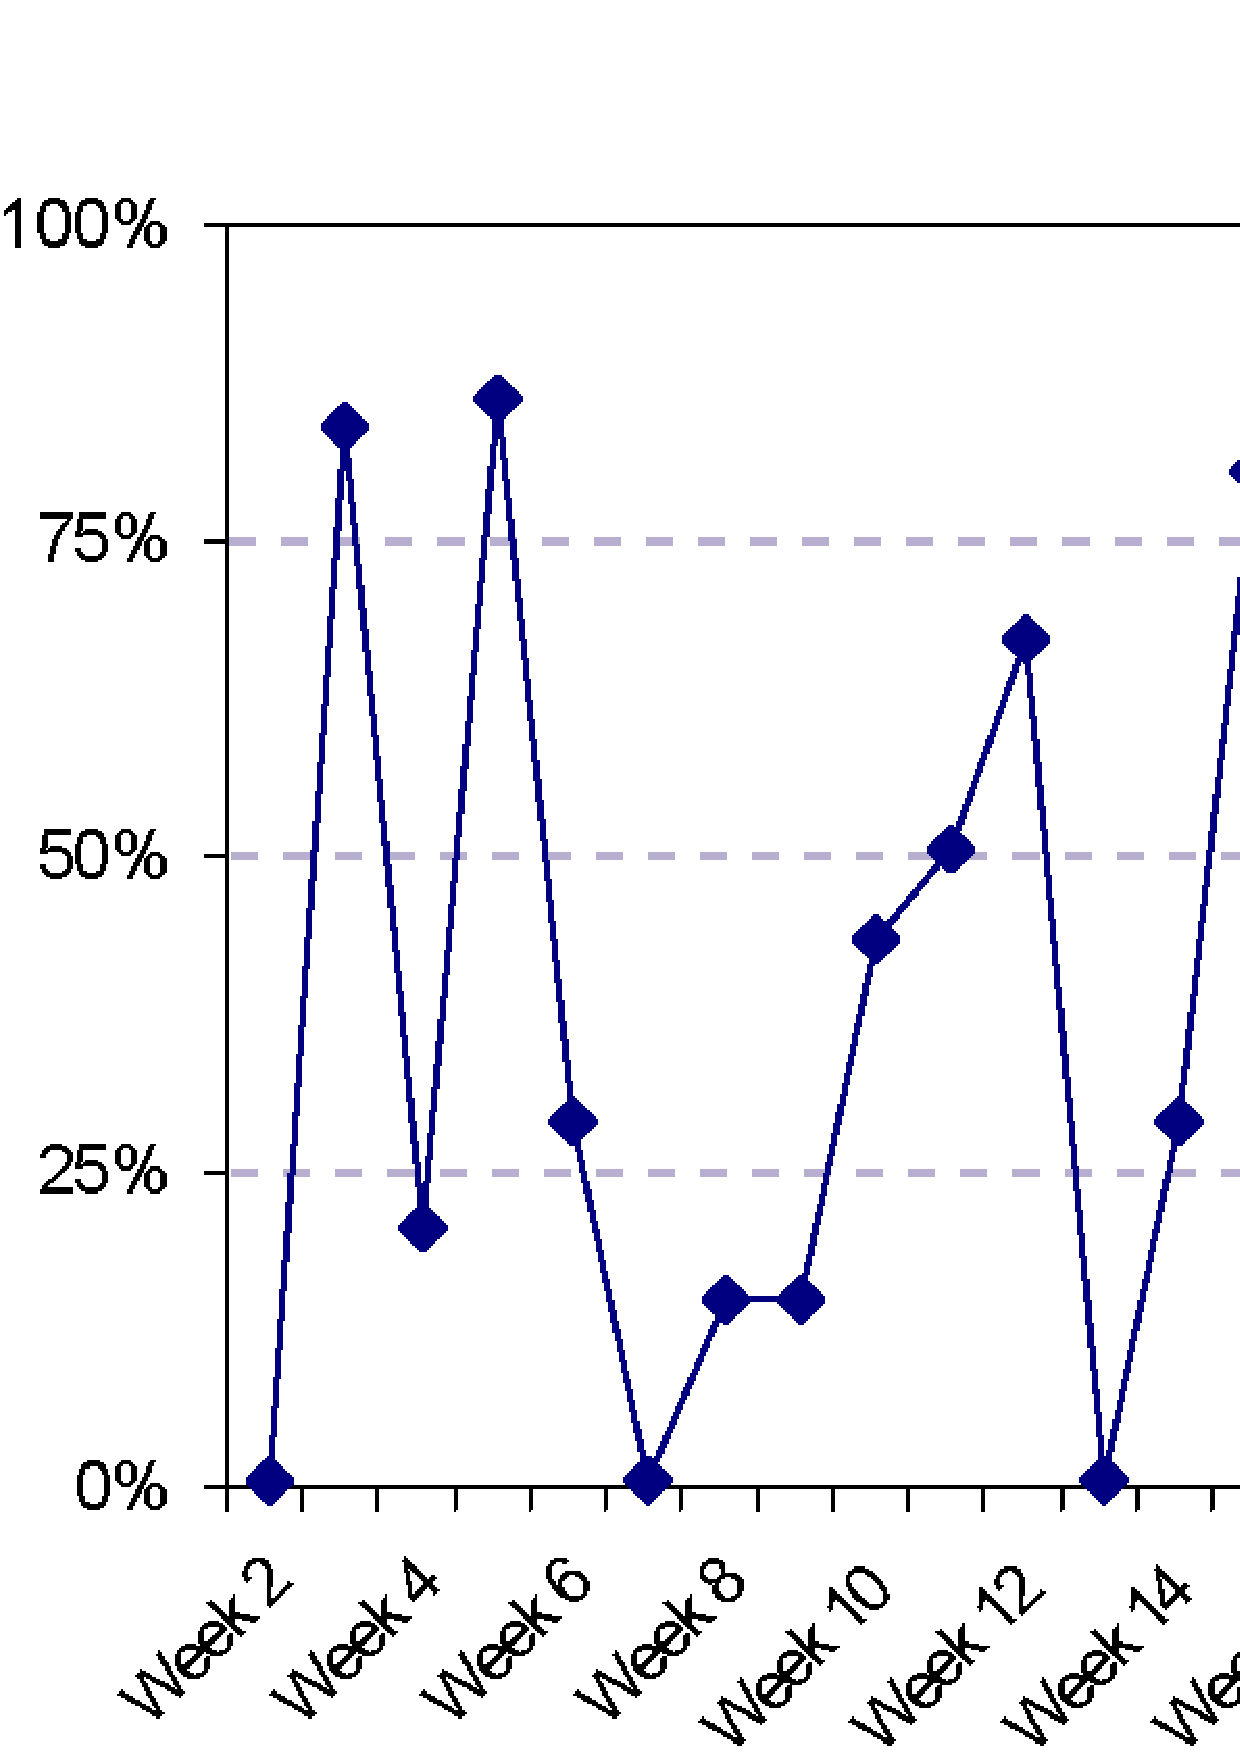
\includegraphics[width=1.00\textwidth]{figures/WeeklyBuildFailureRatio2004}
%  \caption{Weekly Hackystat Build Failure Ratio for the Year 2004}
%  \label{fig:WeeklyBuildFailureRatio2004}
%\end{figure}

\newpage

%In order to reduce the rate of integration build failure, we need to understand more about how, when, and why the builds were failing. To do this, a series of analyses were performed, involving several software project telemetry streams on different aspects of Hackystat development process, such as active time\footnote{Active time is a proxy for developer effort writing or modifying code inside an IDE.}, commit, build, and churn. There were several interesting findings:



%%%%%%%%%%%%%%%%%%%%%%%%%%%%%%%%%%%%%%%%%%%%%%%%%%%%%%%%%
%           S U B   S E C T I O N                       %
%%%%%%%%%%%%%%%%%%%%%%%%%%%%%%%%%%%%%%%%%%%%%%%%%%%%%%%%%

\subsection{Initial Investigation}  \label{EvaluationInCSDL:InitialInvestigation}

Several metrics on different aspects of the development process were used in the initial investigation: 
\begin{itemize}
	\item \textit{Active Time} --- The proxy for developer effort writing or modifying code inside an IDE.
	\item \textit{Commit} --- The commit of a file to a source code repository. 
	\item \textit{Build} --- The invocation of a build tool (Apache Ant in this case) and the build result.
	\item \textit{Churn} --- The lines added and deleted in the source during some period of time.
\end{itemize}


The investigation revealed several interesting findings:

\begin{table}[tbp]
	\centering   
		\begin{tabular}{|c|c|c|c|c|} 
			\hline
			\textbf{} & \textbf{Coding Standard Violation} & \textbf{Compilation Failure} & \textbf{Unit Test Failure} & \textbf{Other Errors} \\
			\hline
			\textit{\textbf{Count}} & \textit{14} & \textit{25} & \textit{40} & \textit{16} \\
			\hline
		  \textit{\textbf{Percentage}} & \textit{14.74\%} & \textit{26.32\%} & \textit{42.11\%} & \textit{16.84\%} \\
			\hline
		\end{tabular}
  \caption{CSDL 2004 Integration Build Failures}
	\label{table:CSDL-BuildFailureCategory-2004}
\end{table}

\begin{itemize}
	
	\item The 95 integration build failures in 2004 could be partitioned into 4 major categories as shown in Table \ref{table:CSDL-BuildFailureCategory-2004}: coding standard violation (14), compilation failure (25), unit test failure (40), and others (16). The 16 ``other errors'' consisted of 8 build script errors, 3 platform errors, and 5 unknown errors. Platform errors refer to the ones caused by external factors, such as network unavailability and operating system failure, which is generally beyond the control of the developers. The unknown errors are the ones that I was unable to assign cause because of insufficient archived information.
% [cumulative stream, showing the type of build fauilure.]

	\item The two Hackystat modules with the most dependencies to other modules had the two highest numbers of build failures, and together they accounted for 30\% of the total failures.
%[Cumulative module level build failure stream here.]
	
	\item The days with build failures had a statistically significant greater number of distinct module commits than the days without build failures. 
%Combinational telemetry chart here, plus statistics.
	
	\item There was no statistical correlation between integration build failure and the number of lines of code committed or the amount of active time spent before the commit. In other words, whether you worked 5 hours or 5 minutes, or whether you changed 5 lines of code or 500 did not change the odds of causing an integration build failure. 
%[Combinational telemetry chart, plus statistics.]
	
  \item There were substantial differences (5 -- 10 fold) between experienced and new developers with respect to their propensity to fail the integration build. 
%[Beyond telemetry capability. do I really want to write code to infer who fails the build? If it's not accurate most of the time, it's useless.]
	
	\item Most integration build failures were confined within single Hackystat module. 74\% of the failures could have been prevented if the developer could test the modules they were working on before committing the changes to the central code repository. A further 6\% could have been avoided if the developer could run a full system test over all Hackystat modules before committing their changes.	
	
\end{itemize}



%%%%%%%%%%%%%%%%%%%%%%%%%%%%%%%%%%%%%%%%%%%%%%%%%%%%%%%%%
%             S U B   S E C T I O N                     %
%%%%%%%%%%%%%%%%%%%%%%%%%%%%%%%%%%%%%%%%%%%%%%%%%%%%%%%%%

\subsection{Initial Hypothesis}

%The initial results yielded a number of interesting hypotheses to improve the build process, such as increasing the support for new developers through pair programming, refactoring modules to reduce coupling and the frequency of multi-module commits. 

Perhaps the most significant finding was that most integration build failures were confined to a single module, and that  74\% -- 82\% of them were actually preventable if the developers could build and test the system on their workstation before committing the changes to the central code repository. Therefore, the simplest process improvement recommendation would be to require all developers to test their modules every time before making a commit. The problem with this recommendation was the large amount of overhead involved. A system test takes at least 10 to 20 minutes depending on the number of modules and the speed of the workstation. %CSDL developers typically perform multiple commits each day. 
Though some commits without testing caused integration build failures, many did not. The cost of productivity loss associated with this naive process change might well exceed the benefit it would bring.
%[ToDo: Can show a telemetry stream here. 2004 info not available, since build sensor was not installed.]

%[ToDo: Requiring system test before the last commit of the day should be feasible.]

The initial analysis also suggested that the causes of the integration build failures were quite complex. They involved developer's familiarity with the system, the actual changes made to the code, the dependency relationships among the modules, etc. However, there was no statistical correlation between build failure and the number of files committed or developer active time. It would be difficult to adopt the traditional approach to build an analytical model to predict the probability of integration build failure in order to forewarn the developers.


The approach to improve CSDL build process in this case study came from the recognition of the following trade-off: 

\begin{itemize}
	\item Reducing the number of integration build failures could increase developer productivity.
	\item Performing local system test could reduce the number of integration build failures at the expense of developer overhead. 
\end{itemize}

As a result, the goal of build process improvement is not to minimize the absolute number of integration build failures. Instead, the goal is to increase the overall developer productivity by making their software development process transparent, providing them with process feedback, and helping them understand plausible causes of integration build failures, so that they could make an informed decision when a local system test would likely to be necessary before committing the changes. 


%\textcolor{red}{[TODO: Copy the telemetry process methodology chart here: process problem detection, hypothesis generation... Customize it to this build problem.]}




%%%%%%%%%%%%%%%%%%%%%%%%%%%%%%%%%%%%%%%%%%%%%%%%%%%%%%%%%
%                                                       %
%                   S E C T I O N                       %
%                                                       %
%%%%%%%%%%%%%%%%%%%%%%%%%%%%%%%%%%%%%%%%%%%%%%%%%%%%%%%%%

\section{Study Participants and Researcher's Role}  \label{EvaluationInCSDL:Role}

I joined CSDL in 2003. Currently CSDL has 6 members. Three of them are Ph.D. students (including me). They are hired as research assistants (0.50 full time equivalence) by Dr. Philip Johnson to develop and maintain the Hackystat framework. At the same time, they are doing their own doctoral research using the framework as a software engineering experimentation tool. The other 3 members are undergraduate students in their final semester working on Hackystat for course credits. They are top students from software engineering classes.

Dr. Philip Johnson is the director of CSDL. He is my dissertation adviser. He is the project manager of Hackystat responsible for major architectural design and scheduling decisions. He also contributes to Hackystat development.

The software project telemetry system used in this case study is designed and implemented by me as part of my dissertation research. It is built on top of the Hackystat foundation, leveraging its generic framework of metrics collection and project management.

The 5 CSDL members (excluding me) and Dr. Philip Johnson (as project lead and developer) are the participants of this case study. Though I am also a member of CSDL and contribute to Hackystat development, I will exclude my development activities from this case study.





%%%%%%%%%%%%%%%%%%%%%%%%%%%%%%%%%%%%%%%%%%%%%%%%%%%%%%%%%
%                                                       %
%                   S E C T I O N                       %
%                                                       %
%%%%%%%%%%%%%%%%%%%%%%%%%%%%%%%%%%%%%%%%%%%%%%%%%%%%%%%%%

\section{Case Study Design and Strategies}  \label{EvaluationInCSDL:Design}

The purpose of this case study is two-fold:

\begin{itemize}
	\item To use software project telemetry to understand and improve CSDL build process.
	\item To evaluate software project telemetry during the process.
\end{itemize}

The second objective is more important than the first one. I want to understand how software project telemetry technology can be applied in a more traditional software development environment such as CSDL with relatively centralized decision-making and close collaboration. I want to know how the developers make use of telemetry information to make process improvement decisions. I want to know their opinions about the technology. I want to find out what works, what doesn't work, and what can be improved.
	
The organization of this section is as follows. 
Section \ref{EvaluationInCSDL:Design:ImproveBuildProcess} elaborates on the steps to improve CSDL build process with software project telemetry.
Section	\ref{EvaluationInCSDL:Design:EvaluateTelemetry} details evaluation strategies.
	
	
	
\subsection{Improving CSDL Build Process}	 
\label{EvaluationInCSDL:Design:ImproveBuildProcess}
	
In order to improve CSDL build process, I will use software project telemetry to collect and analyze relevant process and product metrics, and make the information transparent to the entire development team. I will provide process feedback through both pull style telemetry analysis and push style telemetry alert. The hypothesis is that when the developers are made more aware of their development process and night integration build results, they can become better at deciding when a local system test is likely to be necessary before committing their changes.
%\begin{figure}[p]
%  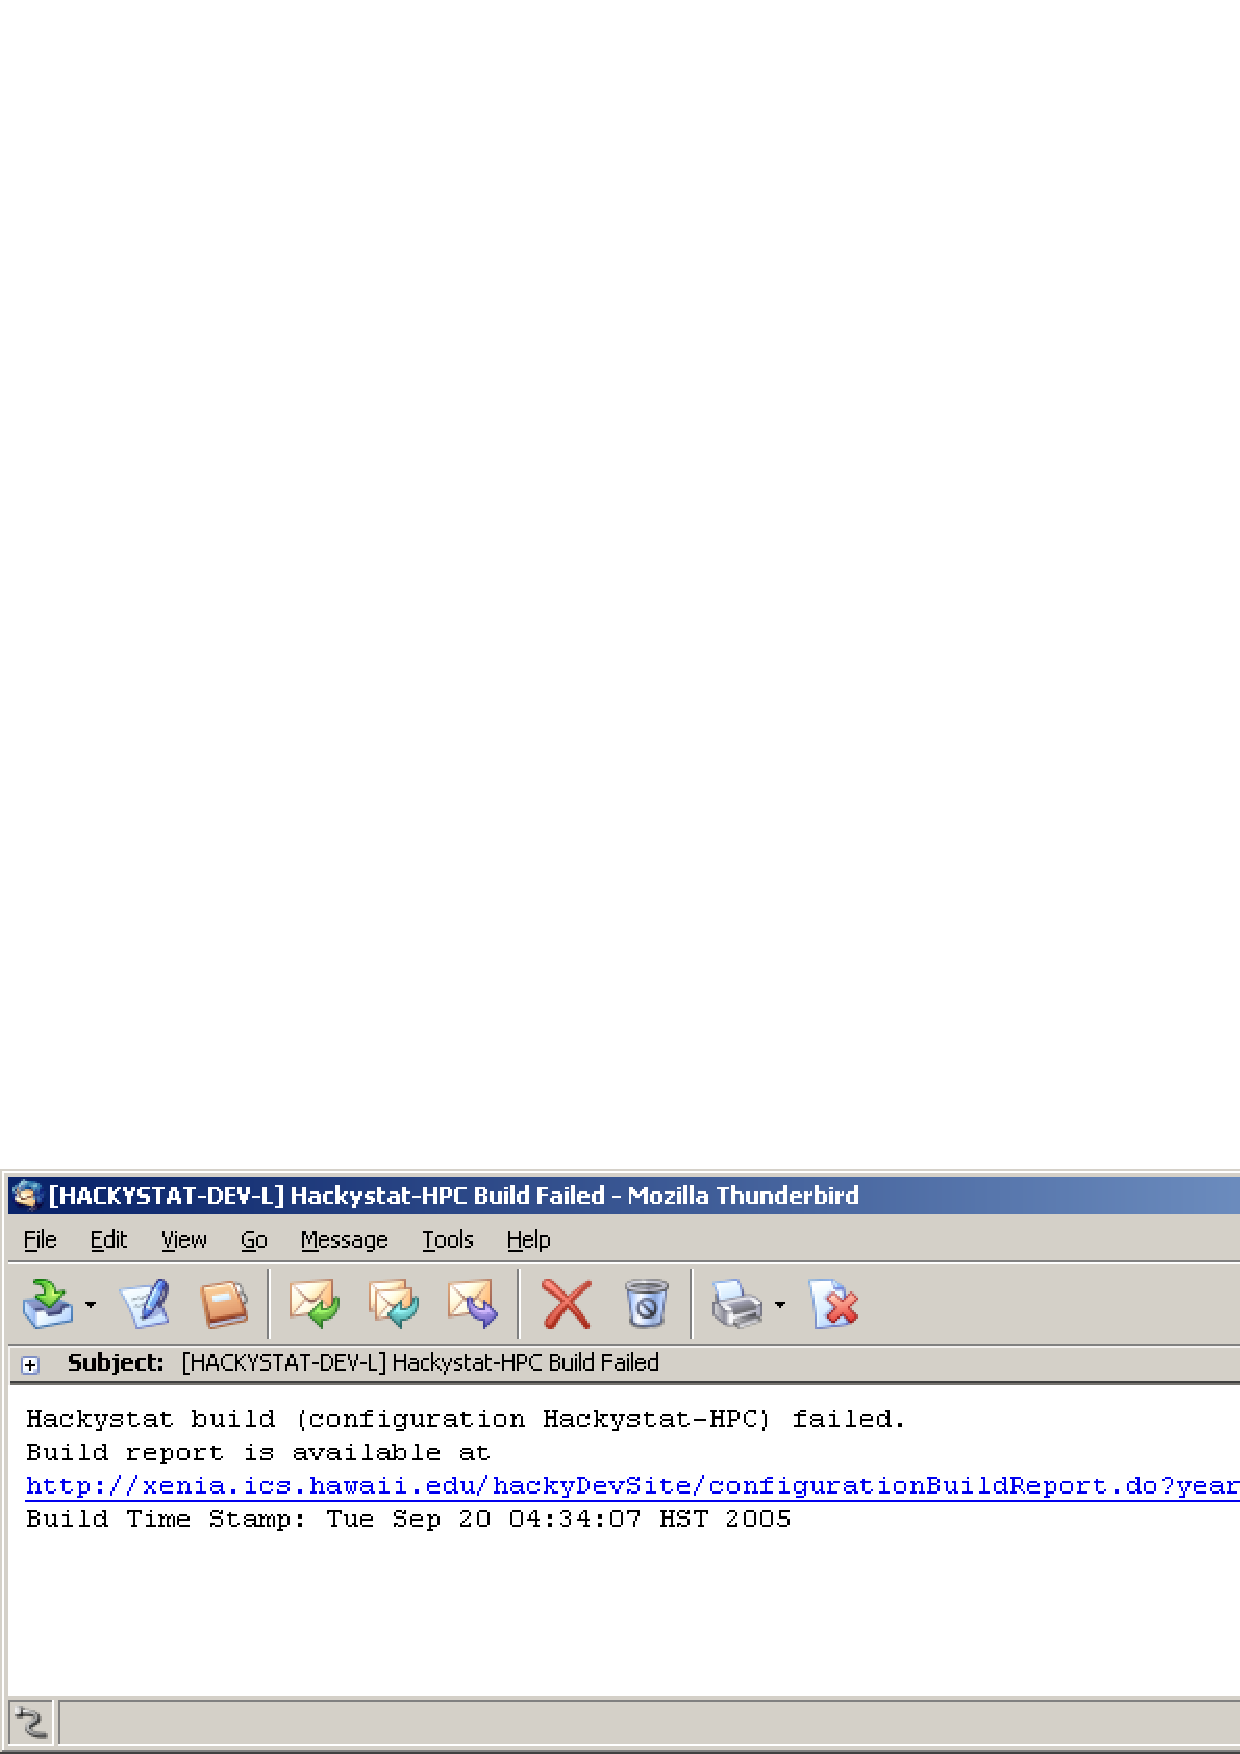
\includegraphics[width=1.00\textwidth]{figures/OriginalBuildFailureEmail}
%  \caption{Current Integration Build Failure Alert Email} 
%  \label{fig:OriginalBuildFailureEmail}
%\end{figure}
%
%\begin{figure}[p]
%  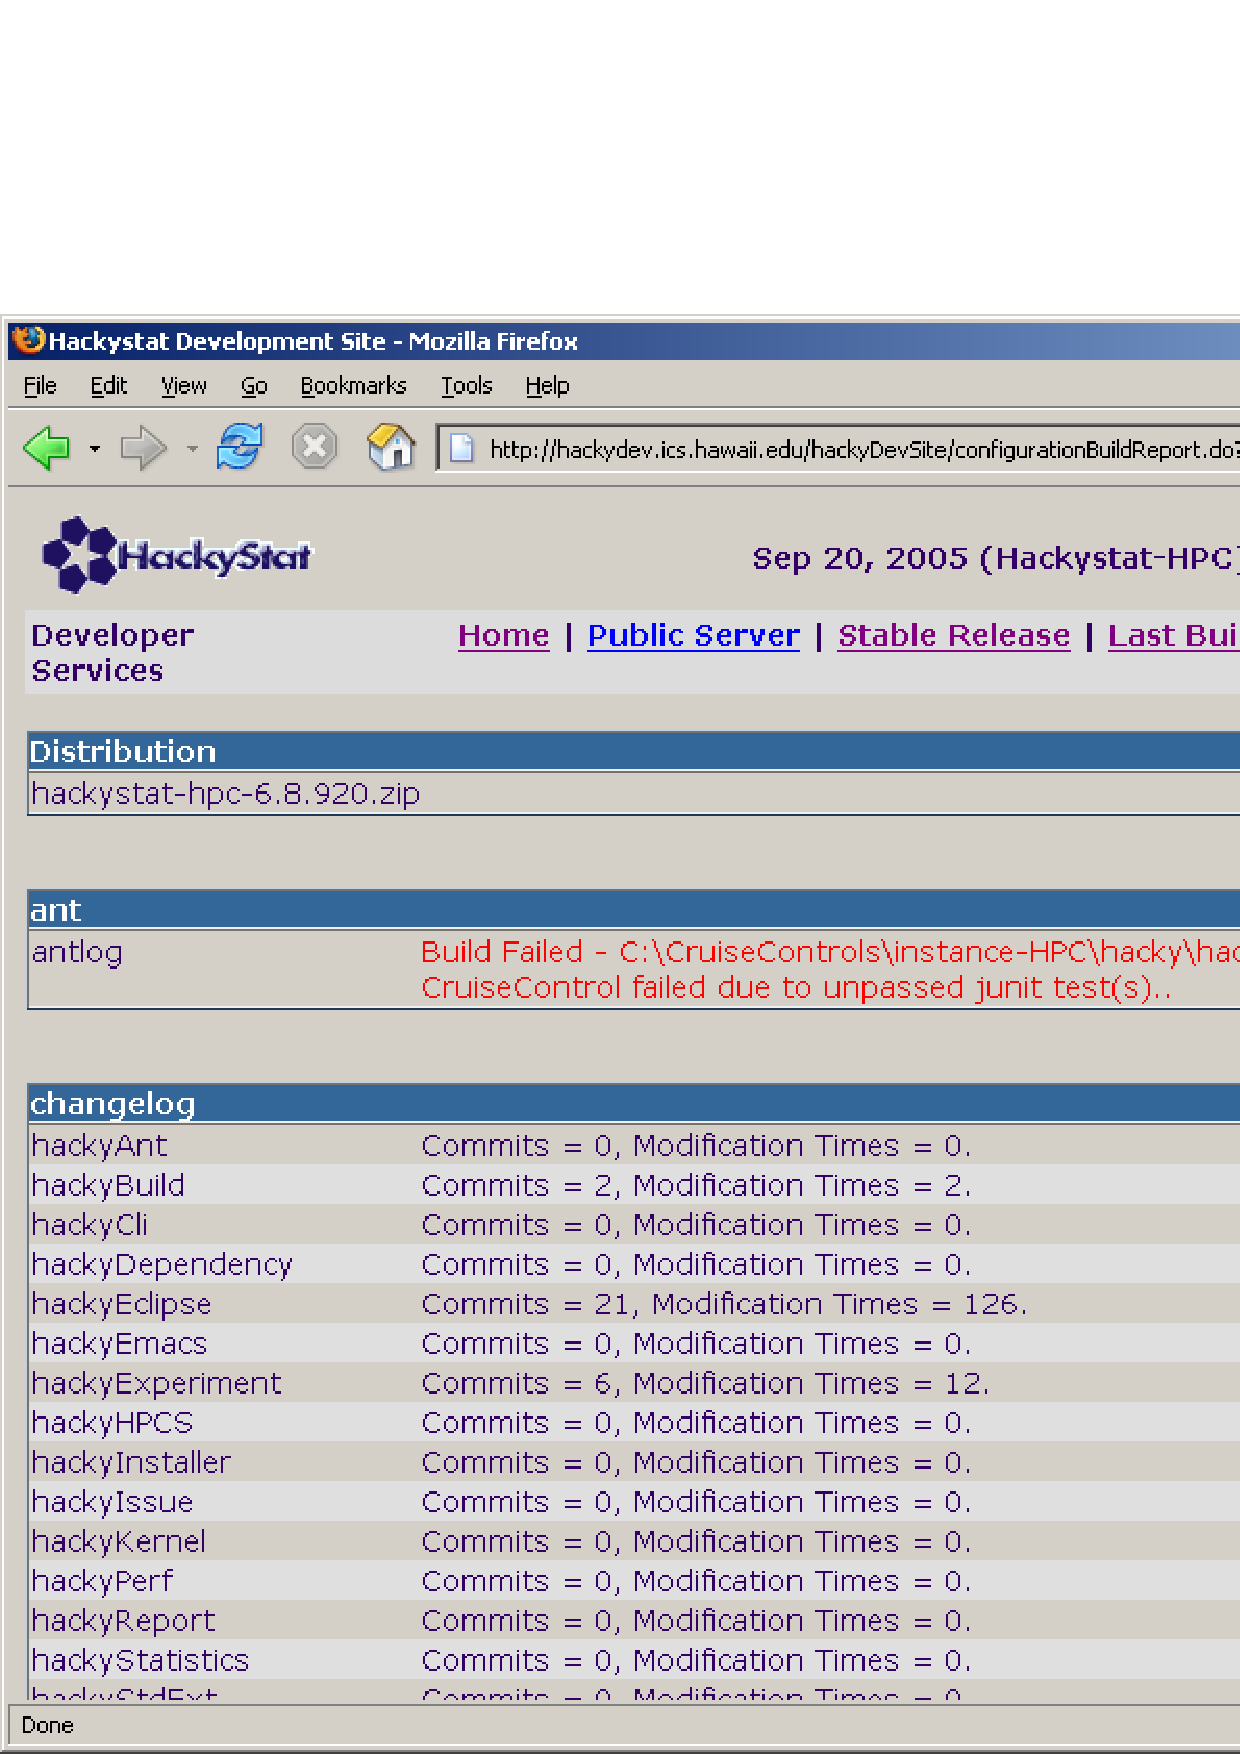
\includegraphics[width=1.00\textwidth]{figures/BuildFailureReport}
%  \caption{Integration Build Report} 
%  \label{fig:BuildFailureReport}
%\end{figure}

The 2004 CSDL build analysis was performed manually which required a tremendous amount of effort. The only information available was the archived email alerts notifying the developers of integration build failures. As a result, I had to checkout the snapshot of Hackystat source code for each day in 2004, simulate the build, and find out where and why the build failed. I spent the entire winter break (1 month) to perform the analysis. 

The manual approach will not work for CSDL members to improve their build process, simply because of the tremendous amount of overhead associated with manual metrics collection and analysis. Fortunately, we can use software project telemetry to automate these time-consuming metrics collection and analysis tasks. As the first step of this case study, I developed a build sensor, which runs on both the integration build server and individual developer's workstation. The sensor collects the following information automatically and unobtrusively: build time, build context (environment information about the build, such as who starts the build, on which computer the build is started, which modules are being built, build target, etc.), and build results (in case of build failure, which module, which file, and which step is the cause of the failure). The build data, combined with other metrics collected by the existing sensors, such as IDE sensor (who is editing which file), CVS sensor (who has committed which file), provide a holistic picture of the entire team's build process.



\subsubsection{Pull Style Telemetry Analysis}

The software project telemetry system, which is first introduced in Chapter \ref{Chapter:Implementation}, will be used in this case study. The implementation contains generic support for telemetry-style software metric analysis such as telemetry definition management and telemetry language interpreter. I will customize the system with an initial set of telemetry streams, based on the analysis of 2004 CSDL integration build metrics, to provide process feedback to CSDL developers. This set may change during this case study as I understand more about the role of software metrics in improving CSDL build process.

The initial set of telemetry streams I plan to implement can be divided into the following categories:

\begin{enumerate}
	\item \textit{Telemetry streams related to integration build failures --- team level}
	
  \begin{enumerate}
	  \item Integration build failure count, with breakdown to failure types such as 
	        coding standard violation, compilation failure, and unit test failure.
	  \item Integration build failure count, with breakdown to modules in which the 
	        failure occurs.
  \end{enumerate}
	
The purpose of these telemetry streams is to inform the developer of the characteristics of build failures such as its distribution over failure type or Hackystat modules, and detect any change in build failure patterns over time.

%Philip and I have also discussed the possibility of writing an intelligent module to infer the developer who caused the failure. 

%The integration build system automates the build of multiple configurations of Hackystat system. Each configuration contains different set of modules to be distributed in different environment. A special configuration ``Hackystat-ALL'' contains all modules in order to ensure there are no incompatibilities between them. In order to eliminate the noise, only the build results of ``Hackystat-ALL'' configuration will be considered in the analysis.
	
		
	\item \textit{Telemetry streams related to local system test and commit --- individual level}
	
  \begin{enumerate}
	  \item Source code commit batch count, with breakdown to commit types (with respect to local system test).
	  \item Local system test count, with breakdown to test target such as source code format check, system compilation attempt, and unit test attempt.
	  \item Local system test count, with breakdown to test result (success or failure).
	  \item Time spent on local system test.
	  \item Integration build failure count caused by insufficient local test.
  \end{enumerate}
	
A significant discovery while analyzing 2004 CSDL build failure metrics was that 74\% to 82\% of them were preventable if the developers could run test over the modules they were working on before committing their changes to the central code repository. As a result, the interaction between the developers' test and commit behavior is an important phenomena to be explored. 

Source code commits are partitioned into 4 types with respect to local system test in this case study:
\begin{itemize}
	\item Commit activity preceded immediately by a full set of successful local system test.
  \item Commit activity preceded immediately by a partial set of successful local system test.
	\item Commit activity preceded immediately by a failed local system test.
	\item Commit activity not preceded immediately by a local test (e.g. editing activity are detected).
\end{itemize}

It is not the design purpose of these telemetry streams to force the developers to run a local system test every time they wish to commit something. Instead, I want to give the developers insight about the relationship between their code commit pattern, local system test pattern, and integration build results, so that they can make trade-off decisions to increase overall development efficiency.

%Since a developer typically makes multiple commits each day, local system test behavior before the last commit is most important from the perspective of integration build result. I will pay special attention to system test behavior before the last commit of the day for each developer. 

%\textbf{Interaction with integration build results: } CSDL is not forcing each developer to test the system before each commit because of the trade-off between additional local testing effort and overall development efficiency. Table \ref{table:CommitBehavior} can help each developer assess the impact of his commit behavior on the result of integration build.
%
%\begin{table}[h]
%	\centering   
%		\begin{tabular}{|c|c|c|c|} 
%			\hline
%			\textbf{} & \textbf{build failed by you} & \textbf{build failed by others} & \textbf{build successful} \\
%			\hline
%			\textbf{Type 1 Commit} & \textit{? times} & \textit{? times} & \textit{? times} \\
%			\hline
%		  \textbf{Type 2 Commit} & \textit{? times} & \textit{? times} & \textit{? times} \\
%			\hline
%		  \textbf{Type 3 Commit} & \textit{? times} & \textit{? times} & \textit{? times} \\
%			\hline
%		\end{tabular}
%  \caption{Developer Commit Behavior}
%	\label{table:CommitBehavior}
%\end{table}
%  
%I will design telemetry streams to help CSDL developers fill out Table \ref{table:CommitBehavior}.
	
	
	
	\item \textit{Telemetry streams related to other relevant information --- individual level}
	
  \begin{enumerate}
	  \item Number of files committed, and number of modules committed.
	  \item Developer active time.
  \end{enumerate}

	   
\end{enumerate}





\subsubsection{Push Style Telemetry Alert}

The current integration build failure email alert contains only a link to the build report. While build reports are excellent source to figure out where the build fails, it does not show process level information. In other words, it helps the developers fix bugs, but does not help them improve their build process.

I will augment the build failure email alert with process level information. It will contain two links: (1) the original link to the build report, and (2) a new link to the build process telemetry analyses. The email will also include summary information about each developer's commit and local system test behavior. More importantly, I will implement a mechanism that will automatically deduce the most likely individual developer who is responsible for integration build failure from telemetry data. Though there would be cases that the mechanism could give erroneous results, the idea is that when the analysis could point fingers to a particular developer, people would have more interest in the analysis and more incentive to avoid build failures.

The summary information will look like:

\begin{verbatim}
  The following alert(s) were triggered today:

  * CSDL Build Analysis Case Study:
  
    Integration build on 08-Oct-2005 
    for hacky2004-all project FAILED.
    [hackyBuild] [JUnit Failure] 
    [Plausible culprit: Developer B]

    Individual Developer Commit and Test Behavior: 
      Total Batches of Commit
      [FullyTested / PartiallyTested / UnTested / FailedTest]
    
      Developer A:  1 [0 / 0 / 1 / 0]
      Developer B:  1 [0 / 0 / 0 / 1]
      Developer C:  1 [0 / 1 / 0 / 0]
      Developer D:  2 [0 / 0 / 2 / 0]
\end{verbatim}


%\begin{table}[h]
%	\centering   
%		\begin{tabular}{|c|c|c|c|} 
%			\hline
%			\textbf{Developer Name} & \textbf{Last Commit Time} & \textbf{Modified Files} & \textbf{Local Testing} \\
%			\hline
%			\textbf{Developer 1} & \textit{11:00pm} & \textit{a.java, b.java} & \textit{passed} \\
%			\hline
%		  \textbf{Developer 2} & \textit{4:00pm} & \textit{c.java} & \textit{failed} \\
%			\hline
%		  \textbf{Developer 3} & \textit{7:00pm} & \textit{d.java} & \textit{no test} \\
%			\hline
%		\end{tabular}
%  \caption{Daily Build Process Summary}
%	\label{table:DailyBuildProcessSummary}
%\end{table}





\subsection{Evaluation of Software Project Telemetry in CSDL}  
\label{EvaluationInCSDL:Design:EvaluateTelemetry}

In order to assess the effectiveness of software project telemetry, I will adopt mixed methods paradigm in this case study collecting and analyzing both qualitative and quantitative information. However, the priority will be skewed toward qualitative information with quantitative data corroborating qualitative findings.

%[Why with priority on qualitative information?]
There are mainly 2 choices to set up the assessment of software project telemetry in CSDL: either a rigid formal experiment or a naturalistic study. I choose naturalistic study over formal experiment in this case study. 

The main advantage of a formal experiment is that controlling of compounding effects leads to maximization of internal validity and that there are relatively straight-forward statistical procedures to determine whether the use of software project telemetry is the cause of build process improvement. However, the reason why the experiment methodology is not chosen is as follows. First, CSDL has 6 developers at the time of this writing, which makes randomized selection of study participants or utilization of control groups practically infeasible. Second, three developers left and three new developers joined the group in the summer of 2005, which makes 2004 integrations build results and process metrics not directly comparable to those that will be obtained in this case study. Third, different developers take responsibility for different modules of Hackystat system with some module inherently more difficult to handle than others. Furthermore, tasks assigned to each developer change over time. These two facts make it hard to compare the process impact between different developers and to control for maturation effects. Perhaps, most importantly, software project telemetry is a young technology, and as such the more pressing need is to explore how the technology can be applied in some software development environment and find out what works and what needs to be improved. Therefore, it is more advantageous to adopt naturalistic approach to provide detailed description of the experience of the application of software project telemetry technology in CSDL, and to use quantitative information to corroborate the findings in qualitative analysis.

Qualitative data will be collected through ethnographic observations, personal diary, and developer interviews; while quantitative data will include integration build results, telemetry analysis invocation records, and individual developer's process metrics. The next section (Section \ref{EvaluationInCSDL:DataAnalysis}) elaborates on data collection and analysis procedures.




%%%%%%%%%%%%%%%%%%%%%%%%%%%%%%%%%%%%%%%%%%%%%%%%%%%%%%%%%
%                                                       %
%                   S E C T I O N                       %
%                                                       %
%%%%%%%%%%%%%%%%%%%%%%%%%%%%%%%%%%%%%%%%%%%%%%%%%%%%%%%%%

\section{Data Collection and Analysis Procedures}  \label{EvaluationInCSDL:DataAnalysis}

This case study will collect both qualitative and quantitative data from multiple sources.
Both types of data will be collected concurrently.

%%%%%%%% Sub Section %%%%%%%%%
\subsection{Qualitative Data Collection}

Qualitative data will be collected through ethnographic observations, personal diary, and developer interviews.


\subsubsection{Ethnographic Observations}

%I am a member of CSDL and I meet with other members almost on a daily basis. 
I will employ ethnography to record the observation of the developers' daily interaction with software project telemetry system and how they make process improvement decisions based on telemetry information. The record of observation will also include contextual information such as the tasks each developer is assigned to, the observed change in the build process, and their comment about software project telemetry.

	
\subsubsection{Personal Diary}

I will keep a personal diary of my interpretation of the observed facts such as daily integration build results, plausible causes of build failures, telemetry analysis results, and the change in each developer's build process. 

      
\subsubsection{Developer Interviews}
	
I will interview the developers on a weekly or bi-weekly basis to find out the impact of software project telemetry on their build process and obtain their comments about the technology. The interview will be carried out in the following steps:
\begin{itemize}
	\item Review past integration build results. Identify the cause for each build failure.
	\item Determine whether each build failure is avoidable or not. Find out whether the responsible developer has performed local test or not. If not, ask the developer whether it is due to neglect, overconfidence, or some other unavoidable reasons.
	\item Go over telemetry analysis results together with the developers. Identify the changes in their process.
	\item Reconcile my own interpretation with the developers' interpretation.
	\item Get developers' opinion about existing telemetry analysis.
	\item Ask developers what can be done to improve telemetry analysis and what other information might be useful. 
\end{itemize}
	
%+ what they want to see, 
%+ what they think when they see the analysis, 
%+ what they did (decision-making) after seeing the analysis 
%  (did the analysis caused them to pay more attention to local build?)
%+ what they think is the impact on their behavior (triangulate with quantitative info)
%+ what they feel that can be improved.
		

%%%%%%%% Sub Section %%%%%%%%%
\subsection{Quantitative Data Collection}

Quantitative data will be collected from the following sources.

\subsubsection{Integration Build Results}
 
The data is collected by the build sensor introducted in Section \ref{EvaluationInCSDL:Design:ImproveBuildProcess}. The sensor is attached to the integration build server collecting build results automatically.
	      

\subsubsection{Individual developer's process metrics}

They are the exactly the same metrics providing process feedback to the developers. These metrics capture information about source code edit, commit, local test, etc. They will be used to assess changes in individual developer's build process.

	      
\subsubsection{Telemetry Analysis Invocation Records} 
	   
The software project telemetry system used in this case study will be instrumented with automatic logging facility. It will record all telemetry analyses invoked by the developers.



%%%%%%%% Sub Section %%%%%%%%%
\subsection{Data Analysis}


Qualitative and quantitative information will be integrated at data interpretation phase with priority given to qualitative information. Quantitative data will be used to corroborate qualitative findings. I will either note the convergence of the findings as a way to strengthen the knowledge claims of the study or explain any lack of convergence that may result.












%%%%%%%%%%%%%%%%%%%%%%%%%%%%%%%%%%%%%%%%%%%%%%%%%%%%%%%%%
%                                                       %
%                   S E C T I O N                       %
%                                                       %
%%%%%%%%%%%%%%%%%%%%%%%%%%%%%%%%%%%%%%%%%%%%%%%%%%%%%%%%%

\section{Threats, Verification, and Validation}  \label{EvaluationInCSDL:Threats}


\subsection{Measurement Validity}

This case study will draw conclusion from both qualitative and quantitative data. Quantitative data are collected automatically either by sensors or through system instrumentation. They all have pretty standard definition, and the risk of measurement validity is very low.

On the other hand, qualitative data used in this case study may suffer from measurement validity. The threat comes from the fact that I am a member of CSDL. Other members might be compelled to comment more favorably about software project telemetry. But there are several mitigating forces:

\begin{itemize}
	\item I am no stranger to other CSDL members, and as a result my ethnographic observation will cause less disturbance on their normal activities.
	\item I have detailed knowledge about the project and have a good understanding about the nature of each developer's task assignment, which gives me great insight into their development process.
	\item Data from multiple source will be cross-validated to assess the effectiveness software project telemetry.
\end{itemize}







%The CSDL project members will serve as a check throughout the entire process of evaluation. An ongoing dialog will be maintained with other members with respect to my interpretations of the metrics and observed facts. 






\subsection{Internal Validity}

Internal validity is related to causality: whether the introduction of software project telemetry in the CSDL development environment does indeed cause the improvement in the build process. Though this case study adopts a naturalistic approach in which compounding factors such as maturation are not controlled, the risk of internal validity threat is mitigated through data triangulation. Data will be collected from multiple sources such as ethnography, personal diary, interviews, process metrics, and server instrumentation. All information will be reconciled and cross-validated at data analysis stage. 





\subsection{External Validity}

CSDL environment resembles traditional software development environment in many aspects. A version control system stores the source code; an issue management system tracks features requirements, bugs, assigns tasks to developers; an integration system builds and tests the project automatically; and code reviews are conducted on a regular basis. However, it is still an academic environment and my have different constraints in software development than industrial environment.

The primary strategy to ensure external validity will be the provision of rich, thick, detailed descriptions of this case study. This way, anyone interested in extending CSDL experience will have a solid framework for comparison.





%%%%%%%%%%%%%%%%%%%%%%%%%%%%%%%%%%%%%%%%%%%%%%%%%%%%%%%%%
%                                                       %
%                   S E C T I O N                       %
%                                                       %
%%%%%%%%%%%%%%%%%%%%%%%%%%%%%%%%%%%%%%%%%%%%%%%%%%%%%%%%%

\section{Expected Results}  \label{EvaluationInCSDL:Results}

The use of software project telemetry will have impact on CSDL build process, though it is hard to tell to what extent the development process can be improved at this stage. However, regardless of the outcome, I will gain experience by applying software project telemetry to solve development process problems. This experience will enhance our understanding of the technology.






%%%%%%%%%%%%%%%%%%%%%%%%%%%%%%%%%%%%%%%%%%%%%%%%%%%%%%%%%
%                                                       %
%                   S E C T I O N                       %
%                                                       %
%%%%%%%%%%%%%%%%%%%%%%%%%%%%%%%%%%%%%%%%%%%%%%%%%%%%%%%%%

%\section{Time Frame}  \label{EvaluationInCSDL:TimeFrame}
%
%I expect to start the case study from Oct 1, 2005. The study will last 5 to 6 months.
%





%%%%%%%%%%%%%%%%%%%%%%%%%%%%%%%%%%%%%%%%%%%%%%%%%%%%%%%%%
%                                                       %
%               G R A V E Y A R d                       %
%                                                       %
%%%%%%%%%%%%%%%%%%%%%%%%%%%%%%%%%%%%%%%%%%%%%%%%%%%%%%%%%


%One of the advantages of software project telemetry is that it enables an experiential approach to information discovery. Multiple telemetry streams, representing different perspectives on development process, are aligned together over the same time period. Though correlation between different telemetry streams does not necessarily indicates causal relationship, it might help us generate process improvement hypothesis.
%
%Current visual representation is intuitive when a human is inspecting telemetry charts visually. However, sometimes numerical statistical information might be more direct. As the first step, I plan to add a correlation table in telemetry analysis expert interface. For example, when a user requests telemetry analysis involving 3 telemetry streams, both visual and numerical information will be presented. The chart will be displayed followed by a statistical correlation table shown below:
%
%\begin{table}[h]
%	\centering   
%		\begin{tabular}{|c|c|c|c|} 
%			\hline
%			\textbf{} & \textbf{Telemetry 1} & \textbf{Telemetry 2} & \textbf{Telemetry 3} \\
%			\hline
%			\textbf{Telemetry 1} & \textit{1} & \textit{0.89} & \textit{0.23} \\
%			\hline
%		  \textbf{Telemetry 2} & \textit{0.89} & \textit{1} & \textit{0.34} \\
%			\hline
%		  \textbf{Telemetry 3} & \textit{0.23} & \textit{0.34} & \textit{1} \\
%			\hline
%		\end{tabular}
%  \caption{Hypothetical Telemetry Stream Correlation Table}
%	\label{table:TelemetryStreamCorrelation}
%\end{table}
%
%From Table \ref{table:TelemetryStreamCorrelation}, it is quite obvious that telemetry 1 and telemetry 2 are correlated.

